\section{Online Contactless Finger Knuckle Identification}

With TRTL loss, the RFNet \cite{liu2020contactless} can outperform state-of-the-art methods. In the previous section, we have estimated its verification and identification performance on different public finger knuckle database, including within-db and cross-db experiments. As for a completely contactless and online finger knuckle identification, the finger knuckle detector is a very important module for automatically detect and segment finger knuckle region. However, as for traditional segmentation algorithm, they cannot correctly segment the finger knuckles in the presence of complex background interference, multiple finger knuckles in the same field of view, obscured finger knuckles or bent finger knuckles.
Meanwhile, as for neural network, the current based on YOLO \cite{redmon2016you}, \cite{redmon2017yolo9000}, \cite{redmon2018yolov3}, \cite{bochkovskiy2020yolov4}, \cite{YOLOv5} and R-CNN \cite{girshick2014rich}, \cite{girshick2015fast}, \cite{ren2015faster}, \cite{he2017mask} series object detection and segmentation approaches cannot simultaneously obtain the angle of finger knuckle and the segmentation with high precision. Especially, the angle of the finger knuckle is a vital factor for identification. If we can get the angle of finger knuckle, we can use angle information to align two feature maps for increasing matching accuracy and efficiency. For solving above problems, we propose rotated bounding box detection based on YOLOv5 model for segmenting and getting angle information.

\subsection{Contactless Finger Knuckle Detection}
\subsubsection{ Rotated Bounding Box Based on YOLOv5}
In order to solve the problem of finger knuckle detection in the real world, we choose to use YOLOv5 model because the YOLO series is famous for its fast detection speed and high accuracy. Especially, the YOLOv5's \cite{YOLOv5} speed can meet our online detection requirements.

\noindent\textbf{Rotated Bounding Box}

\noindent{ However, the YOLOv5 just detect horizontal bounding boxes which cannot offer angle information and will segment a lot of background information. In order to solve these above problem, a rotated bounding box will be predicted instead of horizontal bounding box. As analyzed in this paper \cite{yang2020csl}, the rotated bounding boxes loss will mainly come from angular periodicity and the exchangeability of edges. When use the long side definition of rotated bounding box, it can deal with the exchangeability of edges problem. Meanwhile, using classification task to predict angle can make model easier to train. A periodic coding method called Circular Smooth Label (CSL) \cite{yang2020csl} soft coding can also solve the problem that One-Hot cannot distinguish class relationship. Formula \ref{CSL Function} $g(x)$ is the window function to smooth One-Hot label, and $r$ is a window function of the radius.}

\begin{equation}
    CSL(x)=
    \begin{cases}
        g(x), &\theta-r<x<r+\theta \\
        0   , &\text{otherwise}
    \end{cases}
    \label{CSL Function}
\end{equation}

Furthermore, in this paper, we used the Gaussian function for the Equation \ref{CSL Function} window function, a commonly available function, and used a window radius of 6 to smooth the labels.


\noindent\textbf{Loss function}

\noindent{The original YOLOv5 loss function can have three components. The formula can be simply written as $Loss = CIOU\_Loss + Loss_{conf} + Loss_{class}$. Since the rotated bounding box is based on the modification of YOLOv5, only the angle classification loss is added more. So the total loss function is as expressed in Equation \ref{Loss}, with the addition of $Loss_{angle}$ to YOLOv5 loss function.}

\begin{equation}
    Loss = CIOU\_Loss + Loss_{conf} + Loss_{class} + Loss_{angle}
    \label{Loss}
\end{equation}

\begin{equation}
    \begin{aligned}
        Loss_{angle} = \sum_{i=0}^{S^2}I_{ij}^{obj}\sum_{a{\in}[0,180)}[\hat{P_i(a)}log(P_i(a)) + \\
        (1-\hat{P_i(a)})log(1-P_i(a))]
    \end{aligned}
    \label{Loss_angle}
\end{equation}


\subsubsection{Contactless Finger Knuckle Dataset}
Our task is to detect finger knuckles in the contactless and online scenario, but by understanding current public finger knuckle database, their data are collected at specific conditions such as certain angle, certain light. In this kind of situation, this kind of data cannot represent real images of finger knuckle in real world. In order to address the shortcomings of current public finger knuckle dataset for contactless detection, we use a web crawler to get images from the Unsplash \cite{Unsplash} where the keywords are finger knuckles. The Unsplash is an image site that offers uploads and downloads, and uses a copyright license that allows users to download and use them for free or even for commercial use \cite{unsplashlicense}. We have downloaded 2347 images, there are 738 images without knuckles, and these images can be used as background training, and the rest 1609 images that contain at least one finger knuckle are the positive samples for the network model. In the network training process, we use crawled images, 169 finger knuckle images from the HKPolyU Finger Knuckle Database (V1.0) \cite{fingerknuckledbv1.0}, and 64 finger knuckles images from the HKPolyU Hand Dorsal Database \cite{ContactlessHnadDorsaldb} as for the training set. And we use the rest data as testing set to evaluate performance. The most important part is the data augmentaion which conatains flip, rotation, resize, translate and mosaic.

\subsubsection{Contactless Finger Knuckle Detection}

\noindent\textbf{Detection Performance}

\noindent
The YOLOv4 model predict horizontal bounding box, while the remaining YOLOv5 model predict rotated bounding box with CSL classification, called YOLOv5-CSL. We can see the performance difference between these variations of the YOLOv5 model from the Table \ref{mAP of different model}. Among the downloaded 2580 images, 100 images were randomly selected as the testing set.

\begin{table}[H]
    \centering
    \begin{tabular}{c c c c c c}
        \hline
        Model & \makecell[c]{Inference \\ Time/ms\\ (1024x1024)} & \makecell[c]{Number \\of Layers} & \makecell[c]{${mAP}^{val}$\\0.5} & \makecell[c]{AP of\\ Major \\FK} & \makecell[c]{AP of\\ Minor \\FK}\\
        \hline
        YOLOv5x-CSL & 41.395 & 407 & \textbf{89.9} &\textbf{89.6} & \textbf{90.1} \\
        YOLOv5m-CSL & 36.252 & 263 & 85.7 & 88.9 & 80.4 \\
        YOLOv4 & 25.992 & 161 & 70.7 & 83.6 & 57.7 \\
        \hline
    \end{tabular}
    \caption{Comparison of the accuracy of the different models of the YOLO series for the detection of the finger knuckle.The calculated values of mAP were measured at a detection threshold of 0.4 as well as an IOU threshold of 0.5.}
    \label{mAP of different model}
\end{table}

\textbf{Segmentation Performance}

This section aim to compare quality of finger knuckle between YOLOv5-CSL segmented and dataset offered. Because the segmented finger knuckle on the 3D Finger Knuckle Dataset already have high quality, I mainly test on the Index Finger Knuckle of Hand Dorsal Dataset and the Finger Knuckle Dataset V3 (with deformable).

\begin{figure}[H]
	\centering
	\begin{subfigure}[b]{0.45\linewidth}
		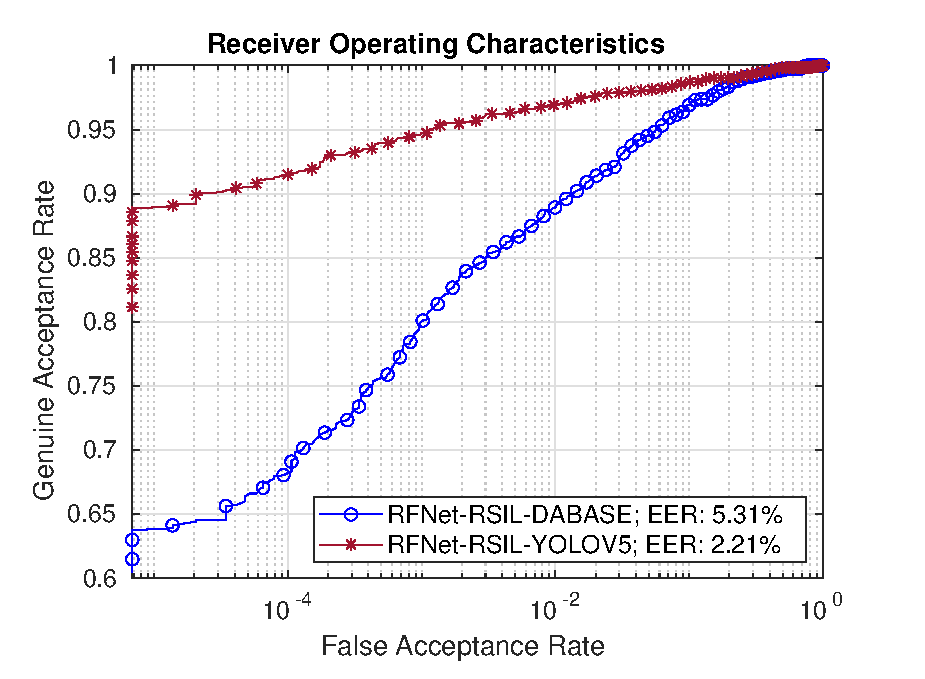
\includegraphics[width=\linewidth]{Figures/yolov5vsdatabase/fkv3-roc_compare_new.eps}
	\end{subfigure}
	\begin{subfigure}[b]{0.45\linewidth}
		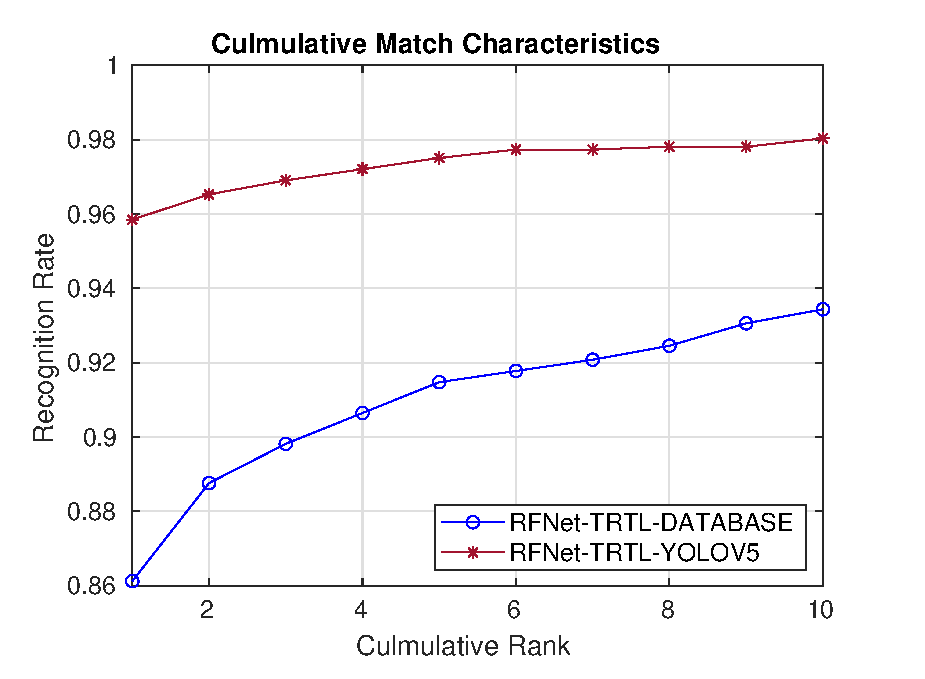
\includegraphics[width=\linewidth]{Figures/yolov5vsdatabase/fkv3-cmc_compare_new.eps}
	\end{subfigure}
	\caption{Compare performance on the Finger Knucle V3 Dataset (with deformable)}
\end{figure}

\begin{figure}[H]
	\centering
	\begin{subfigure}[b]{0.45\linewidth}
		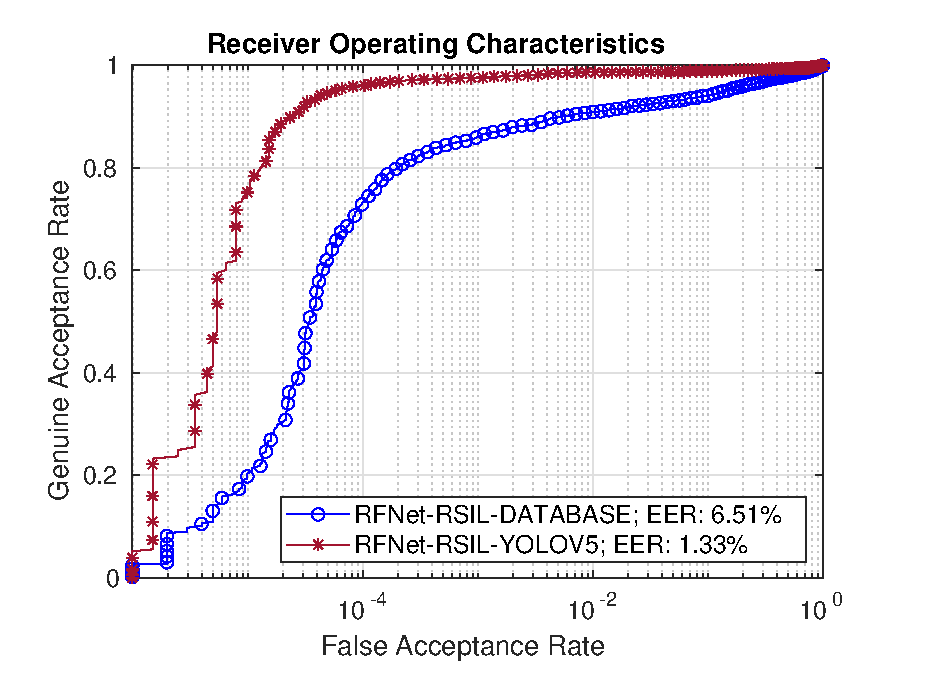
\includegraphics[width=\linewidth]{Figures/yolov5vsdatabase/hd-roc_compare_new.eps}
	\end{subfigure}
	\begin{subfigure}[b]{0.45\linewidth}
		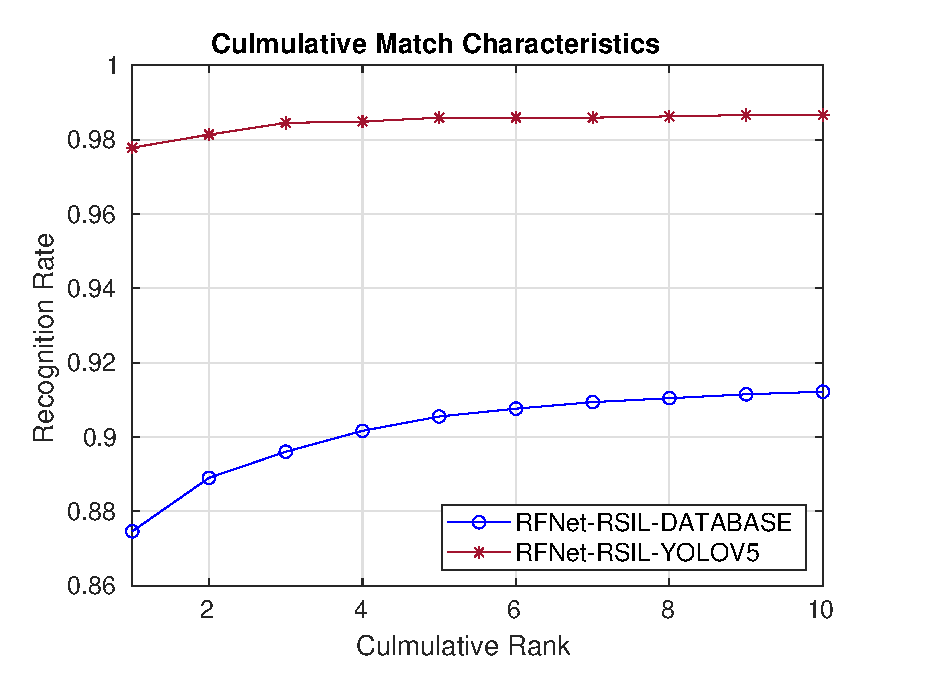
\includegraphics[width=\linewidth]{Figures/yolov5vsdatabase/hd-cmc_compare_new.eps}
	\end{subfigure}
	\caption{Compare performance on the Index Finger of the Hand Dorsal Image Database.}
\end{figure}

From the above figures, we can clearly get the conclusion that quality of segmented finger knuckle of YOLOv5 is better than the segmented finger knuckle of dataset through the ROC curve and CMC curve. Especially on the Hand Dorsal Image Database, the EER value can drop from $6.51\%$ to $1.33\%$. 



 \subsection{Online Contactless Finger Knuckle Identification Performance}
 .............